\documentclass[../main/main.tex]{subfiles}


\begin{document}

\section{January 29th, 2020}
%\subsection{Exact ODE}
\subsection{Phase Plot}
Let us consider ODE's of the form: \[
	\frac{dx}{dt}=f(x)=\dot{x}
.\] 
If we graph $x$ vs  $\dot{x}$ we can get a phase plot, for example:
\begin{figure}[htpb]
	\centering
	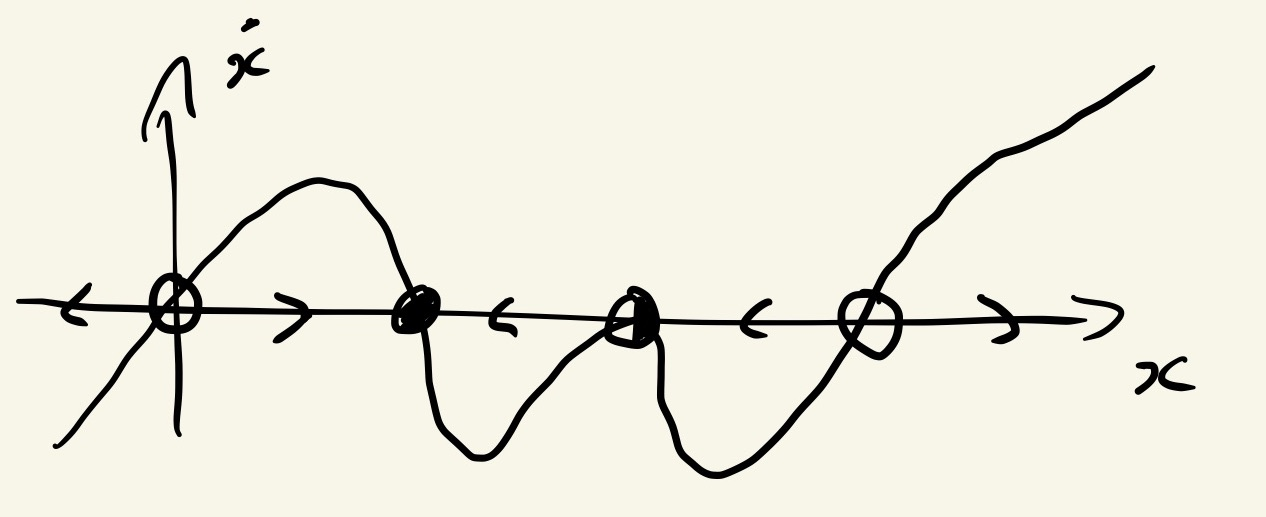
\includegraphics[width=0.8\textwidth]{pp1}
	\caption{Phase plot of $\dot{x}=x(x-1)(x-2)^2(x-3)^{3}$}
	\label{fig:pp1}
\end{figure}

\begin{definition}
	A point where $f(x)=0$ is called an \vocab{equilibrium point}. These equilibrium points can be unstable (empty circle), stable (filled circle), or left/right stable (half filled circle).
\end{definition}

\subsection{Computing Times}
Since $\dot{x} = f(x)$, is separable, since  $dt = \frac{dx}{f(x)}$, we have: \[
	\int^{t_2}_{t_1} dt = \int^{x_2}_{x_1}\frac{dx}{f(x)} \implies t_2-t_1 = \int ^{x_2}_{x_1}\frac{dx}{f(x)}
.\] Which is the time interval between when $x=x_1$ and $x=x_2$.
\begin{example}
	Let us try to compute the period of an object with mass $m$ to travel from one end of a bowl to the other with radius  $R$. TL;DR we get:  \[
		\frac{d\theta}{dt} = \sqrt{\frac{2g}{R}\cos(\theta)} 
	.\] Rearranging gives us: \[
	dt=\sqrt{\frac{R}{2g\cos\theta}} d\theta \implies \int_{-\frac{\pi}{2}}^{\frac{\pi}{2}} \frac{d\theta}{\sqrt{\cos(\theta)} } \approx \sqrt{\frac{R}{2g}} 5.244 
	.\] 
\end{example}
\subsection{Exact Equations}
Whenever you have a function of form $\frac{dy}{dx}=F(x,y)$, you can always rewrite it in the form: \[
	M(x,y) dx+N(x,y)dy=0
.\] This might look familiar, as if we have $f(x,y)=C$, we have:  \[
df = \frac{\partial f}{\partial x} dx + \frac{\partial f}{\partial y} dy=0
.\] As such, we'd like to ask when can $M(x,y)dx + N(x,y) dy=0$ be written as $\frac{\partial f}{\partial x} dx +\frac{\partial f}{\partial y} dy = 0$. It would be great if $M=\frac{\partial f}{\partial x} $ and $N=\frac{\partial f}{\partial y} $, so it's helpful to know when we can do this.

Consider \[
\frac{\partial M}{\partial y} = \frac{\partial }{\partial y} \frac{\partial f}{\partial x} =\frac{\partial ^2f}{\partial y\partial x} \quad \text{and}\quad \frac{\partial N}{\partial x} =\frac{\partial ^2f}{\partial x\partial y} 
.\]  As such, if  \[
\frac{\partial M}{\partial y} =\frac{\partial N}{\partial x} 
,\] then $Mdx+ndy=0$ is called exact. 
\begin{example}
	$2xydx+(x^2-y^2)dy=0$ is exact.
\end{example}
\begin{example}
	$2x^2ydx+(x^{3}-y^2)dy=0$ is not exact.
\end{example}
Note that the two examples differ by a factor $x$, meaning that we have a further condition to determine whether something is exact.
%\begin{figure}[htpb]
	%\centering 
%\begin{tikzpicture}
      %\draw[->] (-0.1,0) -- (4.2,0) node[right] {$x$};
      %\draw[->] (0,-0.1) -- (0,4.2) node[above] {$\frac{dx}{dt}$};
	  %\draw[-] (3.5,-0.1) -- (3.5,0.1) node[below=0.1cm] {\small$C$};
	  %\draw[] node[below=0.01cm] {\small$0$};
	  %\draw[] node[left=0.01cm] {\small$0$};
	  %%\draw[scale=0.5,domain=0:3,smooth,variable=\x,blue] plot ({\x},{\x*\x});
  %\draw[scale=1,domain=-2.3:8,smooth,variable=\x,blue]  plot ({\x},{1/50*1*\x*(3.5-\x)*(7-\x)*(-2-\x)});
    %\end{tikzpicture}
	%\caption{Phase plot of $\frac{dx}{dt}$ vs. $x$}
	%\label{fig:}
%\end{figure}

%\begin{figure}[htpb]
	%\centering 
%\begin{tikzpicture}
	  %\draw[->] (-0.1,0) -- (4.2,0) node[right] {$x$};
	  %\draw[->] (0,-0.1) -- (0,4.2) node[above] {$\frac{dx}{dt}$};
	  %\draw[-] (3.5,-0.1) -- (3.5,0.1) node[below=0.1cm] {\small$C$};
	  %\draw[] node[below=0.01cm] {\small$0$};
	  %\draw[] node[left=0.01cm] {\small$0$};
	  %%\draw[scale=0.5,domain=0:3,smooth,variable=\x,blue] plot ({\x},{\x*\x});
	  %\draw[scale=1,domain=-2.3:8,smooth,variable=\x,blue]  plot ({\x},{\x*(\x-1)*(\x-2)*(\x-2)*(\x-3)*(\x-3)*(\x-3)});
	%\end{tikzpicture}
	%\caption{Phase plot of $\frac{dx}{dt}$ vs. $x$}
	%\label{fig:}
%\end{figure}

\end{document}

